\section{习题}\label{sec:习题02}

\begin{enumerate}
    \item \circleone 利用问题的对称性寻找一种更高效的方法变换轴对齐的边界框:
          因为八个顶点是三个轴对齐基向量与单个顶点的线性组合,所以可以
          用比我们介绍的高效得多的方法\citep{10.5555/90767.90922}找到它们变换后的边界框。
    \item \circletwo 可以通过使用许多非正交块\sidenote{译者注:原文slab。}的交集计算包围物体的更紧致边界,而不是方框。
          扩展pbrt中的边界框表示以允许用户指定任意块构成的边界。
          \begin{figure}[htb]
              \centering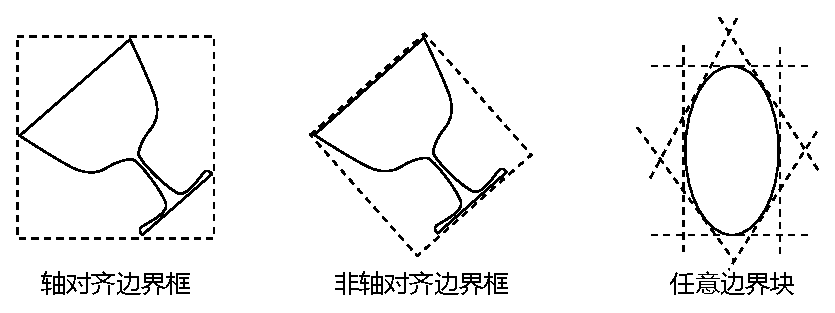
\includegraphics[width=0.8\linewidth]{chap02/Boundingchoices.eps}
          \end{figure}
    \item \circleone 修改pbrt使其像\refvar{Vector3f}{}那样变换\refvar{Normal3f}{},
          并创建因该bug而给出明显错误图像的场景。(完成后别忘了从你的源码拷贝中清除该修改!)
    \item \circletwo 例如,如果一个变换只有平移分量是时变的,则\refvar{AnimatedTransform}{}
          的实现会不必要地计算两个相同旋转之间的插值。修改\refvar{AnimatedTransform}{}
          的实现使其在不需要当前实现中完整一般性的情况下避免这些工作。
          对于适用于你的优化的场景,你观察到了多大的性能变化?
\end{enumerate}

\noindent{\bfseries 第1题解答}\sidenote{译者注:这是笔者根据原文所给参考文献摘录的。}
\begin{algorithm}[htb]
    \SetAlgoNoLine
    \caption{Transform\_Interval\_Box($\bm M,\bm T,\bm A,\bm B$)}
    \KwIn{$3\times3$变换矩阵$\bm M$,平移变换$\bm T$,边界框$\bm A$}
    \KwOut{边界框$\bm B$}
    \For{$i=1\ldots3$}{
    \tcp{从$T_i$处的退化区间开始考虑平移}
    $B_i^{\min}\leftarrow T_i$\;
    $B_i^{\max}\leftarrow T_i$\;
    \tcp{通过计算最小和最大元素与$\bm M$第$i$行的积来求得极值}
    \For{$j=1\ldots3$}{
    $a\leftarrow M_{i,j}*A_j^{\min}$\;
    $b\leftarrow M_{i,j}*A_j^{\max}$\;
    $B_i^{\min}\leftarrow B_i^{\min}+\min(a,b)$\;
    $B_i^{\max}\leftarrow B_i^{\max}+\max(a,b)$\;
    }
    }
\end{algorithm}